%----------------------------------------------------------------------------------------
%	PACKAGES AND OTHER DOCUMENT CONFIGURATIONS
%----------------------------------------------------------------------------------------

\documentclass{article}
\usepackage{amsmath,amsthm}
\usepackage{amsfonts}
\usepackage{fancyhdr} % Required for custom headers
\usepackage{extramarks} % Required for headers and footers
\usepackage{graphicx} % Required to insert images
\usepackage[outdir=./figures/]{epstopdf} 
\epstopdfDeclareGraphicsRule{.pdf}{png}{.png}{convert -density 300 #1 \OutputFile}
\usepackage{pdfpages}
\usepackage{booktabs}
\usepackage{caption}
\usepackage{float}
\usepackage{hyperref}
% Margins
\topmargin=-0.45in
\evensidemargin=0in
\oddsidemargin=0in
\textwidth=6.5in
\textheight=9.0in
\headsep=0.25in 

\linespread{1.1} % Line spacing

% Set up the header and footer
\pagestyle{fancy}
\lhead{\hmwkAuthorName} % Top left header
\chead{\hmwkClass\ : \hmwkTitle} % Top center header
\rhead{\firstxmark} % Top right header
\renewcommand\headrulewidth{0.4pt} % Size of the header rule

\hypersetup{colorlinks=true,urlcolor=blue}
   
%----------------------------------------------------------------------------------------
%	NAME AND CLASS SECTION
%----------------------------------------------------------------------------------------

\newcommand{\hmwkTitle}{Homework\ \#5} % Assignment title
\newcommand{\hmwkClass}{19-704} % Course/class
\newcommand{\hmwkClassInstructor}{} % Teacher/lecturer
\newcommand{\hmwkAuthorName}{Patrick Sheehan} % Your name

%----------------------------------------------------------------------------------------
\begin{document}
\hyperref{https://github.com/patricksheehan/19704}{}{}{Git repository for code for this assignment}

\section{Replication of Baltagi et al. (2000): ``...Replication.R"}
\subsection{Table I replications}
Before delving into the regressions, I first set up the data set as a panel data frame in R using \verb|pdata.frame()|. Since the data is captured over time and across states, each data point is indexed by a state and year. Baltagi et al. (2000) briefly mentions using "real" dollars. To achieve this, I used the provided \verb|cpi| variable to adjust dollars of each year to a base year of 1983. Overall results are contained in Table \ref{Replication}

\subsubsection{OLS}
To replicate the OLS (complete pooling) regression, I used \verb|plm()|, R's panel data regression function, with the model specified\footnote{Specified is a strong word...} by Baltagi et al. (2000):
\begin{align}
\ln(C_{it}) = \alpha + \beta_0\ln(C_{i(t-1)}) + \beta_1\ln(P_{it}) + 
		   \beta_2\ln(Y_{it}) + \beta_3\ln(Pn_{it})
\end{align}

\subsubsection{OLS with time dummies}
To replicate row 2, I added time dummies to the complete pooling regression using the \verb|factor()| function. The updated regression model is:
\begin{align}
\ln(C_{it}) = \alpha + \beta_0\ln(C_{i(t-1)}) + \beta_1\ln(P_{it}) + 
		   \beta_2\ln(Y_{it}) + \beta_3\ln(Pn_{it}) + \beta_4 D_t
\end{align}
Where $\beta$ is a coefficient row-vector and $D_t$ is a column vector of time dummy variables.

\subsubsection{Within model}
To replicate row 4, the within model regression, I used two methods. First, I kept the year dummies and used \verb|plm()|'s "within" model regression option (as opposed to the other models which were simply "pooling" regressions). Second, I used \verb|lm()| with a LSDV model specification which included dummies for both year and state. The Within model math specification is too long to fit on one line, but involves mean-centering each point of interest to remove unobservable, time-invariant properties of the data. The LSDV model is simply:

\begin{align}
\ln(C_{it}) = \alpha + \beta_0\ln(C_{i(t-1)}) + \beta_1\ln(P_{it}) + 
		   \beta_2\ln(Y_{it}) + \beta_3\ln(Pn_{it}) + \beta_4 D_t + \beta_5 D_i
\end{align}
Where $\beta_5$ and $D_i$ are again row/column vectors respectively.

\subsubsection{Results}
My replication results for Table I of Baltagi et al. (2000) is shown below in my Table \ref{replication}.

\begin{table}[H]
\centering
\caption{Replication of Table I from Baltagi et al. (2000)}
\label{replication}
\begin{tabular}{@{}  l r r r r @{}}
& $\ln C_{i(t-1)}$ & $\ln(P_{it})$ & $\ln(Pn_{it})$ & $\ln(Y_{it})$  \\\midrule
OLS & 0.973 & -0.083 & 0.016 & -0.032 \\
OLS with $D_t$ & 0.963 & -0.122 & 0.034 & -0.012 \\
Within & 0.830 &  -0.292 & 0.035 & 0.107 \\
\bottomrule
\hline
\end{tabular}
\end{table}

Comparing with Baltagi et al. (2000), my coefficients seem to align with the ``Short-run" coefficients of Table I. The largest standardized deviation between the two tables is the OLS coefficient for $ln(Pn_{it})$ in which my regression estimated 0.016 where Table I from Baltagi et al. (2000) has a value of 0.024. I could not match the long-run coefficients.

\subsection{Ability to replicate}
I found it extremely difficult to go from Baltagi et al. (2000)'s model description to the close-ish estimates above. While it was clear what variables they used, it was not clear how those variables manifested in each regression. Above all, there was no mention of "short run" and "long run" anywhere in the paper other than in the results table. This relates to reproducibility because it is clear that Baltagi et al. (2000) have not adequately described their model such that it can be replicated.\\

The value of reproducibility lies in the reduction of false or misleading results. Whether intentional or not, results which are either inaccurate or are not adequately tied to a specific model provide no insight. Both lead to people putting undue trust in a result.\\

While providing runnable code is a good step (and shows exactly what you did), this is not enough to make results reproducible. Code can become complex easily, but the underlying math usually requires less interpretation. In light of this, I believe strict and literal model specification without undefined variables or manipulations is necessary to make results truly reproducible.

\subsection{OLS coefficient interpretation} 
Assuming the OLS model corresponds to the first row of both my Table \ref{replication} and Table I from Baltagi et al. (2000), the coefficients can be interpreted as:\footnote{all else equal}
\begin{itemize}
\item  $\ln C_{i(t-1)}$
\begin{itemize}
\item We expect after a 1\% increase in the number of cigarette packs sold in state $i$ in one year (per capita) that the the number of cigarette packs sold in state $i$ the year after will increase by 0.97\%
\end{itemize}
\item  $\ln(P_{it})$ 
\begin{itemize}
\item We expect that a 1\% increase in the price (\$1983) of a pack of cigarettes in state $i$ in a year to decrease the number of cigarette packs sold (per capita) in the state by about 0.083\% in that year.
\end{itemize}
\item  $\ln(Pn_{it})$
\begin{itemize}
\item We expect that a 1\% increase in the minimum price (\$1983) of a pack of cigarettes in states which neighbor state $i$ in a year to increase the number of cigarette packs sold (per capita) in state $i$ by about 0.016\% in that year.
\end{itemize}
\item  $\ln(Y_{it})$
\begin{itemize}
\item We expect that a 1\% increase in the amount of disposable income (\$1983) in state $i$ in a year will decrease the amount of cigarette packs sold (per capita) in state $i$ by 0.032\% in that year.
\end{itemize}
\end{itemize}

\section{Extension}
\subsection{Five stories}
The five stories are:
\begin{itemize}
\item Data summary
\item Conditional distribution
\item Forecasting
\item Statistical inference
\item Causal inference
\end{itemize}

Of the five stories, I think data summary and conditional distribution are the most important to tell. The data summary story is crucial because it lays the foundation for the models and tools we use to make more powerful assertions about the data. Similarly, the conditional distribution story should drive or at least inform the functional form for our model. As my dad always said: ``the truth lies in the disaggregation of data". These stories are as disaggregated as our analysis gets.\\

From my limited experience, it seems as though the data summary and causal inference stories are the most neglected. Most papers don't discuss the peculiarities of the data or where the data might limit the analysis, maybe because these might expose weaknesses of the analysis. For the latter, it might be the case that the analysis cannot dictate causality, and so it is left out of the results to be determined elsewhere. Alternatively, causality may not be a focus of the analysis if prediction is the end goal.\\

I often confuse statistical inference and causal inference because both are focused on using the data to make statements about things outside the data, whether it be a physical relationship or a population from which we think the data are drawn.\\

With respect to data analysis, humans have a disadvantage in two major areas: we can't instantaneously count more than five objects and we have no inherent ability to think probabilistically. On the other hand, as is frequently mentioned in class, humans have great pattern-recognition abilities. While data summary and conditional distributions mostly involve more than five pieces of information, histograms and scatterplots allow us to take masses of data and collect them at low-levels so that we can process them as shapes. I believe these two stories, with those tools, come most naturally to us.\\

The stories we are expected to tell depend on the context and purpose for the data.  In my field, the only thing that matters is minimizing the generalization error, or the error we expect from our model when trying to predict outcomes on random test data. In some cases, outcomes are not observable\footnote{So-called ``unsupervised learning"}, so error minimization becomes even more subjective. Thus for the work I will (likely) end up doing, the only story that I'll be expected to tell is the forecasting story. The data summary and conditional distribution stories only serve the purpose of informing the model.

\subsection{Log transform for dependent variable: ``...Log.R"}
To determine whether the log transformation is appropriate for the dependent variable, cigarette sales in packs per capita for a state at a given time, I used the Box-Cox function with the LSDV model (row 4) to see if the 95\% confidence interval around the MLE includes the log transform. The Box-Cox estimate plotted against log-likelihood is shown below in Figure \ref{boxcar}. While the log transform is not within the bounds of the confidence interval, one might say that it's ``close enough". I think that it is commonly used because, other than when Box-Cox suggests a substantively different transformation, it is the easiest transformation to perform and interpret. Like Matlab, the log transform doesn't make inherent sense, but it benefits from widespread use.

\begin{figure}[H]
\centering
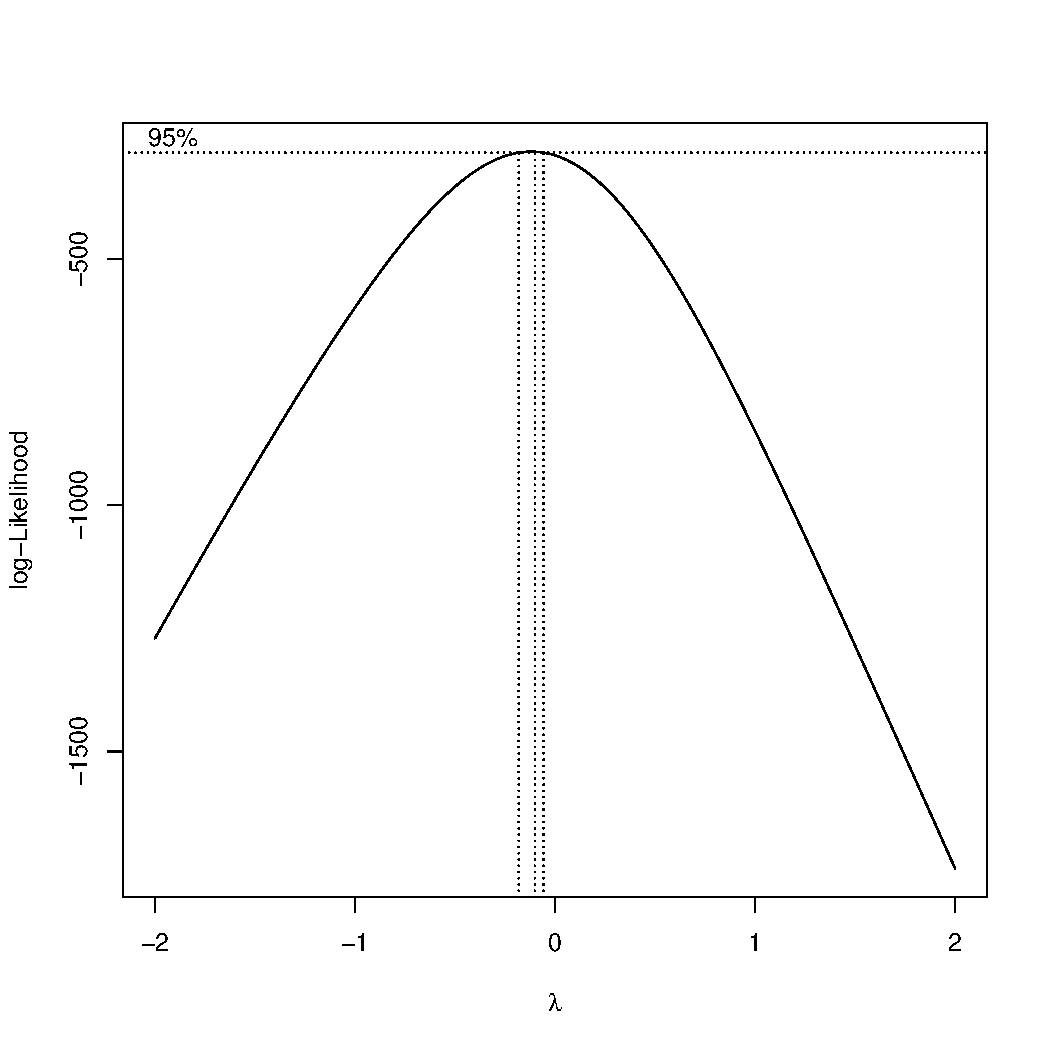
\includegraphics[width = 4in]{figures/BoxCox.pdf}
\caption{Box-Cox log-likelihood plot for cigarette sales per capita}
\label{boxcar}
\end{figure}

The LSDV/Within model is makes the most sense in the context of this problem since we expect both time-invariant and state-invariant properties to have an impact on cigarette sales. One particularly important unobserved property which is prevalent on both levels is the population within each state. While there is some degree of population change over the years, for the most part we expect the same people to live in a state year to year. 

\subsection{Log transformation for independent variables: ``...Log.R"}
To determine whether the log transform is appropriate for the independent variables, I again examined the LSDV model and constructed component plus residual plots for the model as is (with the log transforms) to see if they would show an appropriate linear relationship with our logged dependent variable, sales. The results were created using R's \verb|crPlots()| function and are shown in Figure \ref{caplets}. The results are promising, showing general linear trends for each independent variable in the model with a smoothing line which is also fairly linear for each.

\begin{figure}[H]
\centering
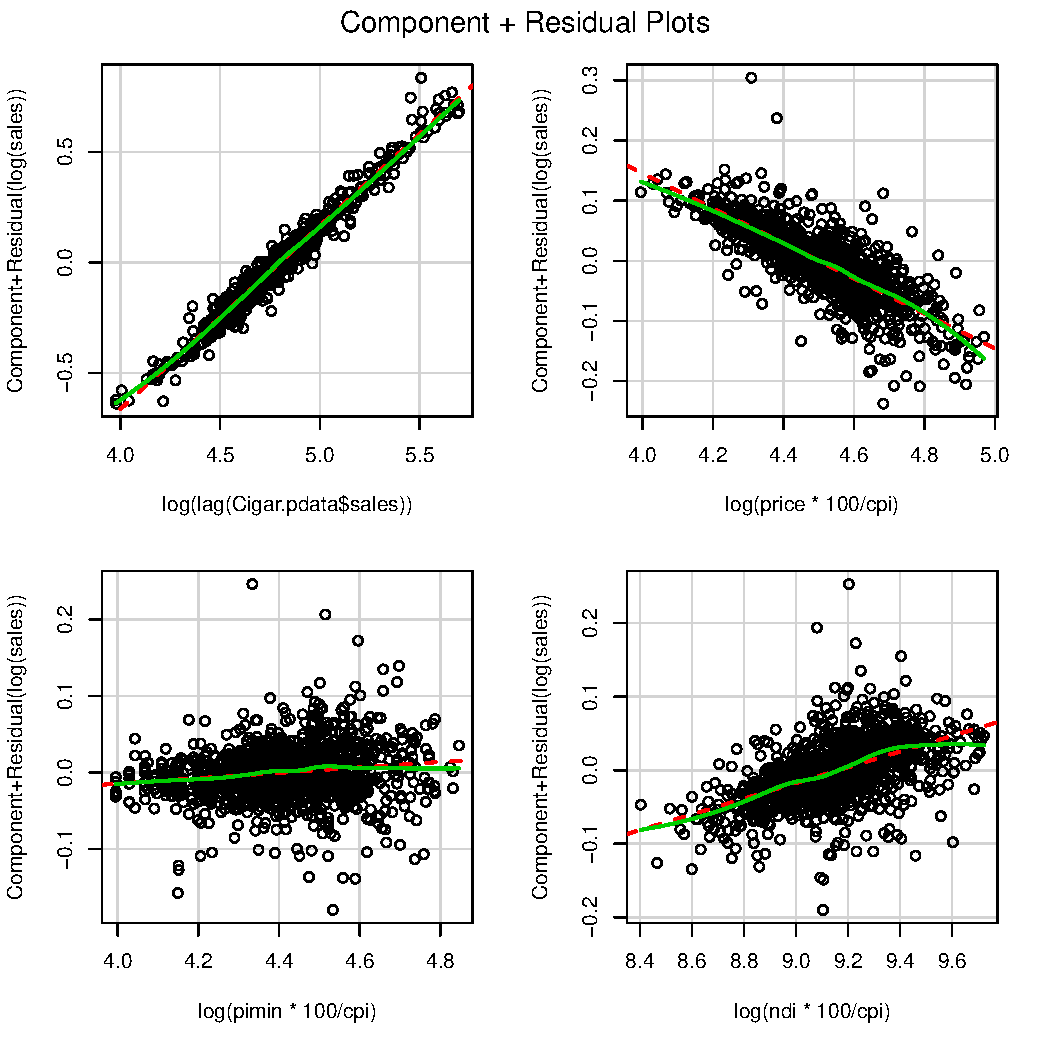
\includegraphics[width = 4in]{figures/CR.pdf}
\caption{Component plus residual plots for each independent variable in the LSDV/Within model}
\label{caplets}
\end{figure}

If one plot suggested a non-log transform, this would indicate issues for the rest of the plots since the component plus residual relationship depends on correct specification of the other regression parameters. In this case, since all the CR plots look OK, we're safe for now. Of course, it could be the case that both all log-transformed independent variables and all untransformed independent variables are both reasonable for the model. In this case, preference of log or non-log depends on how we wish to be able to interpret the coefficients.

\subsection{Residuals: ``...Residuals.R"}
For each model I used the \verb|fitted()| and \verb|studres()| functions to plot the jackknife residuals against the fitted values to look for heteroskedasticity and high influence points. Heteroskedasticity could indicate omitted variable bias or an incorrect model specification where as high influence points could have potentially harmful influence on the regression line if the underlying reason for regression is not to weight outliers more than a standard point. Handling heteroskedasticity could come in the form of a dependent or independent variable transformation to a different functional form, or an added set of variables which may have been omitted in the original model. If high influence residuals are unnatural to the purpose of the model (maybe prediction is the only goal) then ``robust regression" or optimizing for the least absolute deviations is a possible fix.

\subsubsection{OLS model}
The result for the OLS model is shown in Figure \ref{ols residuals}. Overall, there seems to be no general trend for the data, though a few data points are both far from the center of mass and have high residual values, indicating that they may have undue influence on the regression.

\begin{figure}[H]
\centering
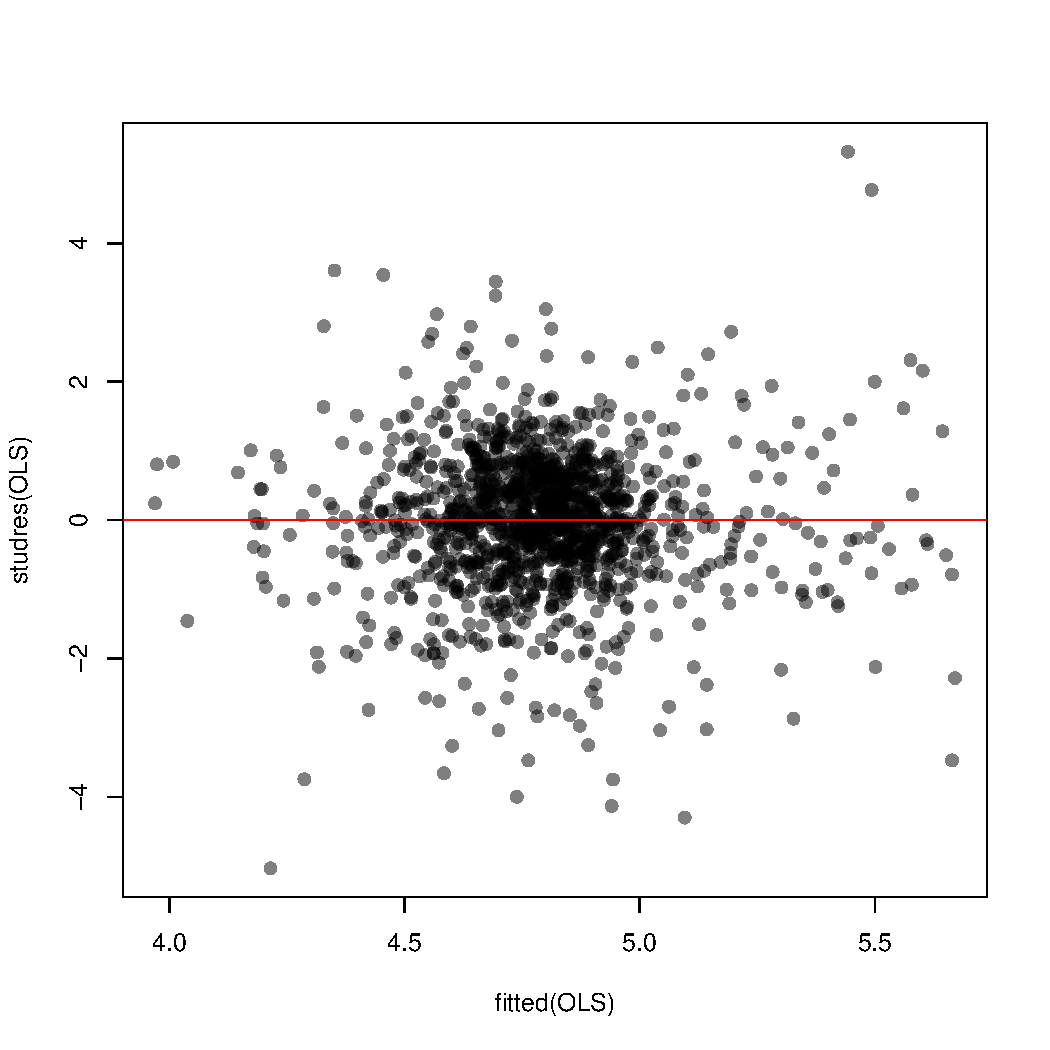
\includegraphics[width = 4in]{figures/residuals1.pdf}
\caption{Residuals vs. fitted values for OLS model}
\label{ols residuals}
\end{figure}

\subsubsection{OLS with time dummies model}
The result for the OLS with time dummies model is shown in Figure \ref{ols time residuals}. Again, no heteroskedastic error pattern emerges, and again a few points appear to have high influence on the regression.

\subsubsection{Within transformation model}
Finally, the result for the within/LSDV model are shown in Figure \ref{within residuals}. Yet again, no clear heteroskedastic pattern is present and yet again we observe that some points have potentially high influence. To be more thorough about examining the influence of these points, I would look at the Cook's D of the jackknife residuals for each model.

\begin{figure}[H]
\centering
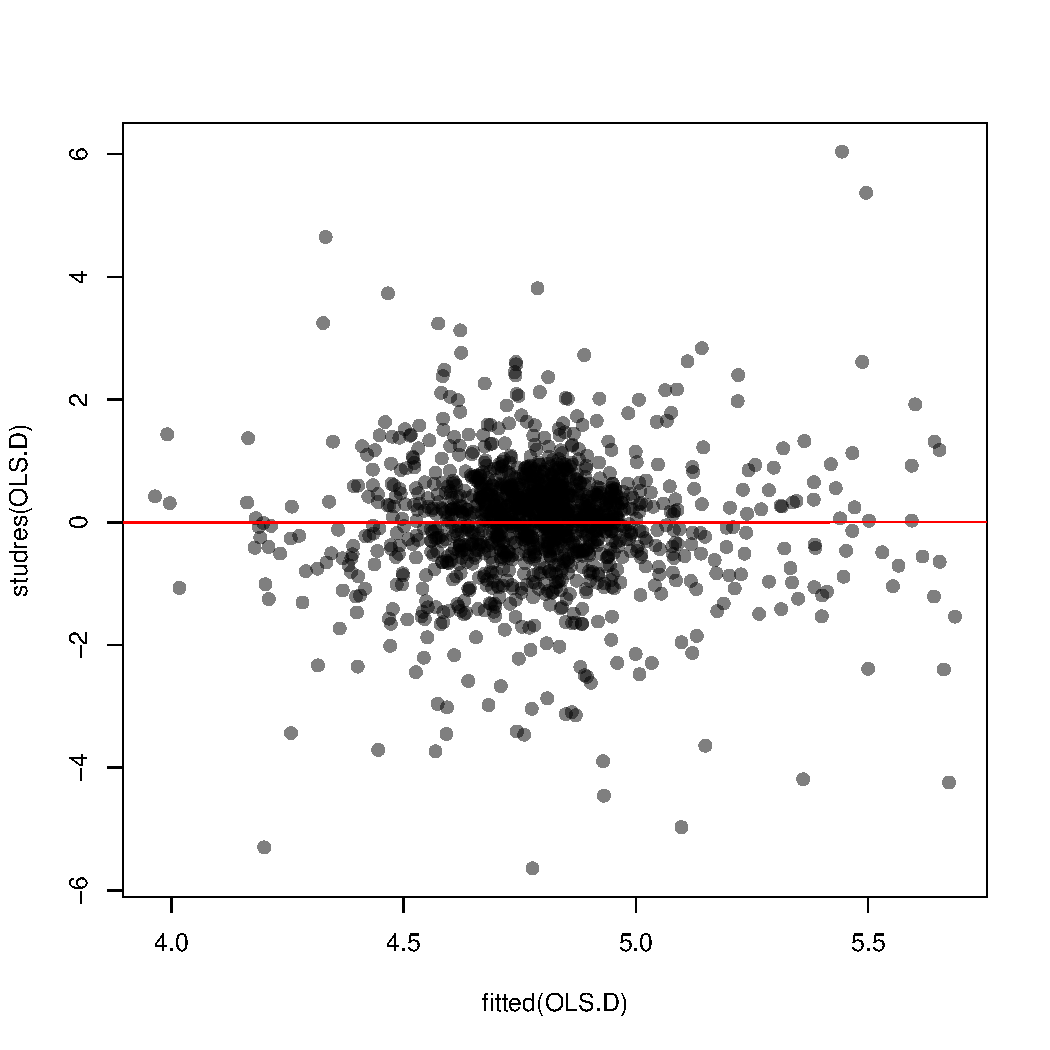
\includegraphics[width = 4in]{figures/residuals2.pdf}
\caption{Residuals vs. fitted values for OLS + $D_t$ model }
\label{ols time residuals}
\end{figure}

\begin{figure}[H]
\centering
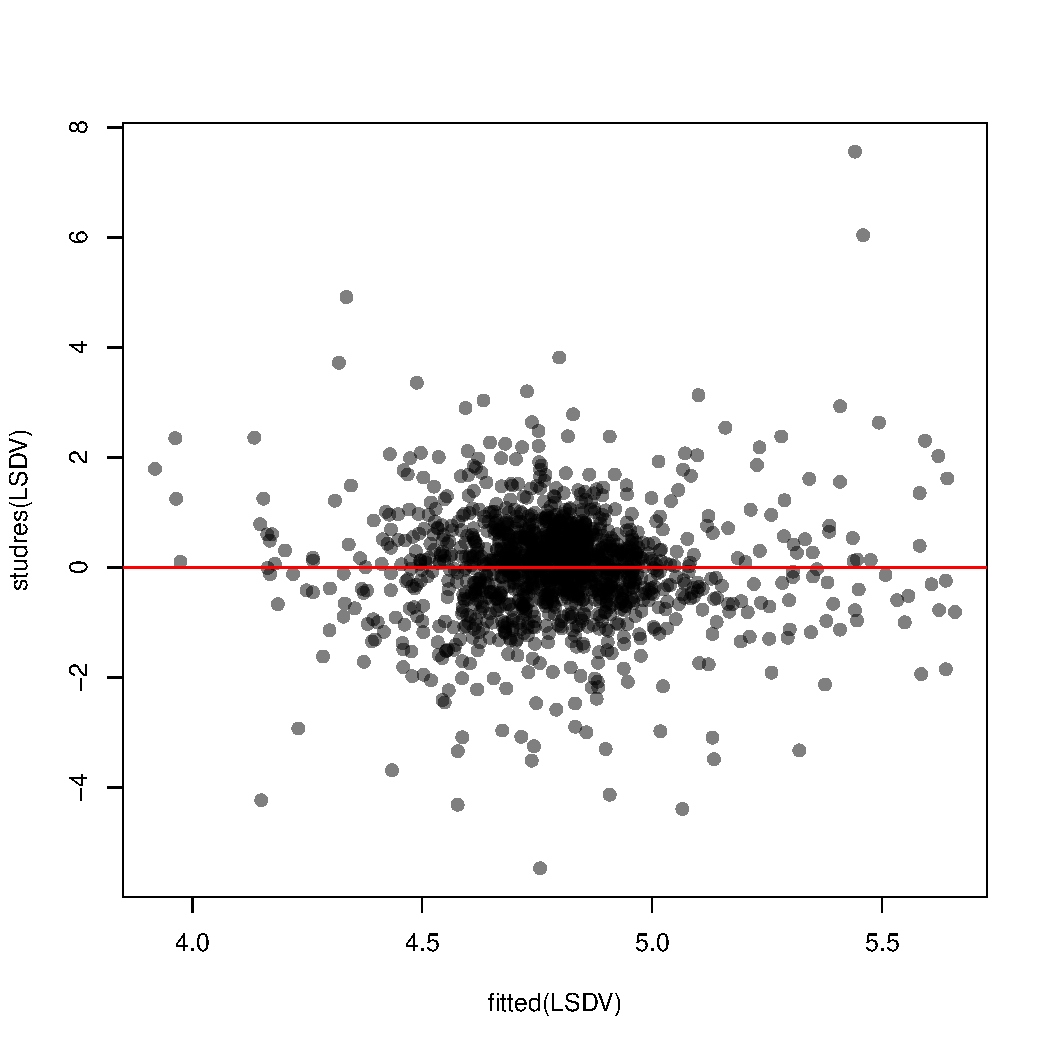
\includegraphics[width = 4in]{figures/residuals3.pdf}
\caption{Residuals vs. fitted values for Within/LSDV model}
\label{within residuals}
\end{figure}

\subsection{Partial pooling of the Within model: ``...Partial.R"}
To conduct a partial pooling version of the Within/LSDV model, I switched to the \verb|lmer()| function in the "arm" package which allows for partially pooled intercepts by state and time. The results for the random effects are shown in Table \ref{random} and the results for the fixed effects are shown in Table \ref{fixed}

\begin{table}[H]
\centering
\caption{Random effects for partially pooled version of the Within model}
\label{random}
\begin{tabular}{@{}  l c @{}}
& \textbf{Variance} \\\midrule
state  & 2.816$\times 10^{-4}$\\ 
 year   & 5.579 $\times 10^{-4}$\\
residual & 1.255 $\times 10^{-3}$\\
\bottomrule
\hline
\end{tabular}
\end{table}

As shown in Table \ref{random}, the state-level intercept variance is about half the year-level intercept variance. In the context of the observation-level error variance (the residual variance), we would need about twice the number of observations within a year to predict better than the information across all years and about four times the number of observations on a state to predict better than the information across all states. 

\begin{table}[H]
\centering
\caption{Fixed effects for partially polled version of the Within model}
\label{fixed}
\begin{tabular}{@{}  r r r r @{}}
 $\ln C_{i(t-1)}$ & $\ln(P_{it})$ & $\ln(Pn_{it})$ & $\ln(Y_{it})$  \\\midrule
 0.892 &  -0.225 & 0.055 &  0.037\\
\bottomrule
\hline
\end{tabular}
\end{table}

The fixed effects for the no pooling within model (Table \ref{replication}) and partial pooling within model (Table \ref{fixed}) are directionally similar, but different nonetheless. In comparison with the no pooling model, the partially pooled model has a smaller disposable income coefficient and it seems as though that effect has been spread to the other coefficients which are all larger in the partially pooled model. \\

My intuition is that the no pooling model would be a better choice for this application. This is because we don't have an issue with an imbalanced distribution of observations (we have the same amount of observations for each time period and the same number of observations for each state). Furthermore, the purpose of the within model is to attempt to remove the time-invariant properties of each state and time period. The theoretical basis for this impact is complicated when we partially pool because the partially pooled intercepts have essentially absorbed portions of the time-invariant properties. If the underlying assumption that states effects are separable from the time effects and vary randomly is not founded, we've re-introduced errors which are correlated with omitted variables.

\subsection{Exogeneity}
\subsubsection{Contemporaneous exogeneity}
In the case of each model, we can assess whether or not contemporaneous exogeneity holds by examining the component plus residual plots and the residuals vs. fitted values plots. While the residual plots for each model did not show any clear trend, this does not give us equal confidence in each model for contemporaneous exogeneity.\\

We expect that the Within model will best establish contemporaneous exogeneity because the fixed effects are explicitly modeled. We are still concerned, however, with possible interactions between states in a single time period which are not modeled.\\

Next, we expect that the OLS with time dummies model will hold reasonably well since time trends of the regressors are modeled with varying time intercepts. Yet unlike the Within model, this model does not account for time invariant properties within state which omitted by the model and thus while the residual plots give no warning signs, we are less confident that contemporaneous exogeneity holds.\\

Finally, we have no reasonable expectation that contemporaneous exogeneity holds with the plain OLS model. The residual plot in Figure 3 indicates no issues, but again we have second order uncertainty in what between state and within state omitted variables might be picked up by our regressors.

\subsubsection{Backwards exogeneity}
Assessing backwards exogeneity is difficult because we include a lagged dependent variable (sales) which is itself a function of the lagged independent variables. So in the status quo we aren't sure whether or not the coefficient of the lagged dependent variable is correlated with the errors in the current time, $t$, or if it is just picking up a connection between the lagged regressors and the future dependent variable value. Likewise if we remove the lagged dependent variable and include lagged independent variables, the reverse is true where we an unsure whether or not we're picking up a correlation with the errors or with the dependent variable. To resolve the issue we could employ instrumentation, but I decided that was too involved :).

\subsubsection{Forward exogeneity}
Since each of the three models explicitly includes a lagged dependent variable, we are fairly confident that forward exogeneity holds. This is because any unmodeled aspect of the dependent variable in time $t-1$ which has an impact on a future time will be captured by including the lagged dependent variable in the model. This holds equally for all three of the models because regardless of whether or not the modeled portion of the dependent variable includes carrying intercepts for time or states, both the unmodeled and modeled attributes are included in the dependent variable inherently. An instance in which we would doubt that forward exogeneity holds is if we believe that a time-lagged effect is "sharp" meaning that a policy implemented in time $t$ has absolutely no effect until time $t+k$ where $k > 1$.

\subsection{Including policies in the model}
Baltagi et al. (2000) handles policies with ``a vector of year-specific, state-invariant variables" which I assume are dummy variables which indicate whether or not the policy had been implemented by year $t$.\\

We can't use difference-in-differences to measure the effect of each policy because the policies included by Baltagi are all national and thus are implemented across all states at the same time. This prevents us from creating pseudo control and treatment groups amongst the panel data observations. In order to construct a difference-in-differences estimate, we would need data on states where the policies were not implemented, at least for a time after the policies were implemented in other states.\\

Supposing we had such data, we would set up our regression to include $Z_t$ from Baltagi as linear regressors to indicate when we are in a period after the policy was enacted. We would also include an indicator variable for each policy which would indicate whether or not the policy was implemented in state $i$ before time $t$. Finally, we would include an interaction term with both of these indicator variables.

\subsection{Forecasting: ``...Forecasting.R"}
For each model, to forecast log cigarette sales in each state in 1992 I:
\begin{itemize}
\item  trained the models with all the previous data
\item created test data with the 1992 data
\item replaced the year with 1991 because we have not estimated intercepts for 1992
\item predicted the log sales for 1992 with the test data
\item found the residuals
\item computed the RMSE
\end{itemize}

The results are shown in Table \ref{Forecast} below.

\begin{table}[H]
\centering
\caption{}
\label{Forecast}
\begin{tabular}{@{}  l c @{}}
 & \textbf{RMSE} \\\midrule
OLS & 1.7 $\times 10^{-3}$\\
Within & 2.5 $\times 10^{-3}$\\
\bottomrule
\hline
\end{tabular}
\end{table}

While we might expect the Within model to perform better, the RMSE I found was higher than that of OLS. This is insufficient evidence to make a predictive performance comparison, however, because we have only tested for a single year. Since we used all but one year to train the model, we expect high variance in our prediction results. Furthermore, to decide how this prediction error relates to which model we think is more appropriate depends on our use for the model. If we take the prediction error at face value, we might conclude that while the Within model is more complex, it performs worse, and is thus over-fitting the data. However, the reasons for the added complexity in the Within model is to assist us with issues in causality, removing omitted time-invariant variables that we have not (and in some cases cannot) observe. So if the goal is to use the model for prediction, the forecasting story tells us that OLS or a less-complex model is the way to go. But if we care at all about establishing causality or statistical inference, judgements based on this single prediction for the value of the model will be misleading.

\subsection{Robust standard errors}
As specified, I got the homoskedastic errors (which are simply the within model standard errors) using \verb|summary()| on the Within regression object. To find the heteroskedasticity robust errors, I used \verb|plm()| to construct the Within model then used \verb|coeftest()| with the "white1" method. Finally, to get the serial-correlation robust standard errors I used the same R function with the "arellano" method. The results are shown in Table \ref{ses} below.
\begin{table}[H]
\centering
\caption{Standard errors for the Within model}
\label{ses}
\begin{tabular}{@{} l r r r r @{}}
 & $\ln C_{i(t-1)}$ & $\ln(P_{it})$ & $\ln(Pn_{it})$ & $\ln(Y_{it})$  \\\midrule
homoskedastic & 0.0126 & 0.0231 & 0.0266 & 0.0233 \\
heteroskedasticity robust & 0.0197 & 0.0284 & 0.0285 & 0.0268 \\
serial-correlation robust & 0.0254& 0.0327 & 0.0309& 0.0362  \\
\bottomrule
\hline
\end{tabular}
\end{table}

From Table \ref{sed}, an interesting trend is that the errors are strictly increasing for each independent variable as we go from the homoskedastic errors to the more robust errors. This suggests that our errors might infact be homoskedastic and that robust errors do not help us. The population that we are using our "robust" errors to make inferences to is not totally clear. Since we're making predictions across years and states, our population may be any state at any time. Since there's no way we can sample representatively from time, since we cannot observe the future, trying to make inferences with standard errors seems unnecessary outside of looking at how different SEs compare.

\end{document}
